
\subsection{O Envelope} % (fold)
\label{sub:o_envelope}

\subsubsection{Gás do Balão}

	Existem duas possibilidades para a escolha do gás do balão cativo, o gás hélio e o gás hidrogênio. A seguir são apresentadas duas tabelas contendo as características físicas dos gases que podem ser escolhidos para o balão. Nas tabelas \ref{tab:caracHelio} e \ref{tab:caracHidro} as características do hélio e do hidrogênio são tiradas da empresa \textit{Gama Gases}.  

	\begin{table}[H]
		\centering
		\begin{tabular}{|c|c|}
			\hline
			\rowcolor[HTML]{FFFFFF} 
			{\color[HTML]{000000} \textbf{Propriedades}}          & {\color[HTML]{000000} \textbf{Valores Numéricos}}                                    \\ \hline
			Densidade absoluta, gás a 101,325kPa a 0 ºC.           & 0,1785 $Kg/m^3$                                                                         \\ \hline
			Densidade crítica                                     & 0,5307 $Kg/m^3$                                                                       \\ \hline
			Densidade relativa, gás a 101,325 kPa a 0 ºC,(ar = 1). & 0,138                                                                                \\ \hline
			Fator crítico de compressibilidade                    & 0,305                                                                                \\ \hline
			Fórmula                                               & 4He                                                                                  \\ \hline
			Massa Molecular                                       & 4,002602                                                                             \\ \hline
			Pressão crítica                                       & \begin{tabular}[c]{@{}c@{}}229 kPa ; 2,29 bar; 33,2 \\ psia;,2,261 atm.\end{tabular} \\ \hline
			Viscosidade, gás a 101,325 kPa a 26,8 ºC.              & 0,02012 mPa x s; 0,02012 cP.                                                         \\ \hline
			Volume específico a 21,1 ºC 101,325 kPa                & 6030,4 dm3/ kg; 96,6 ft3/ Ib                                                         \\ \hline
		\end{tabular}
		\caption{Características do Hélio}
		\label{tab:caracHelio}
	\end{table}


\begin{table}[H]
	\centering
	\begin{tabular}{|c|c|}
		\hline
		\rowcolor[HTML]{FFFFFF} 
		{\color[HTML]{000000} \textbf{Propriedades}}          & {\color[HTML]{000000} \textbf{Valores Numéricos}}                                     \\ \hline
		Densidade absoluta, gás a 101,325kPa a 0ºC.           & 0,08235 $Kg/m^3$                                                                         \\ \hline
		Densidade crítica                                     & 0,0310 $Kg/m^3$                                                                         \\ \hline
		Densidade relativa, gás a 101,325 kPa a 0ºC,(ar = 1). & 0,0695                                                                                \\ \hline
		Fator crítico de compressibilidade                    & 0,305                                                                                 \\ \hline
		Fórmula                                               & H2                                                                                    \\ \hline
		Limites de inflamabilidade no ar.                     & 4,0-75\% (por volume).                                                                \\ \hline
		Massa Molecular                                       & 2,01588                                                                               \\ \hline
		Pressão crítica                                       & \begin{tabular}[c]{@{}c@{}}1297 kPa; 12,97 bar; 188,1 psia;\\ 12,80 atm.\end{tabular} \\ \hline
		Temperatura de auto-ignição.                          & \begin{tabular}[c]{@{}c@{}}844,3 K; 571,2 ºC; \\ 1060 ºF.\end{tabular}      \\ \hline
		Volume específico a 21,1 ºC, 101,325kPa.         & 11967,4dm3/kg; 191,7ft3/lb.                                                           \\ \hline
	\end{tabular}
	\caption{Características do Hidrogênio}
	\label{tab:caracHidro}
\end{table}

	O gás hidrogênio a primeira vista é mais vantajoso pois é mais leve que o hélio, sua densidade relativa ao ar é de 0.0695 enquanto que a do hélio é de 0.138, e apresentam um fator crítico de compressibilidade iguais. Porém o hidrogênio possui a característica de ser inflamável, enquanto que o hélio é conhecido por ser um gás inerte. Tendo em vista a segurança dos usuários do estacionamento e dos funcionários responsáveis pela manutenção do balão, a exposição ao sol e a possíveis, porém improváveis,  descargas elétricas o hélio se mostra a opção mais vantajosa.

	\subsubsection{Material do Envelope}

	Segundo Yajima (2009), a maioria dos balões atmosféricos são feitos de filme de polietileno. A espessura dos envelopes dos balões usados pela NASA variam de 7 a 90 micrometros dependendo da altitude, funcionalidade, tempo de atividade e peso da payload e etc. Desta forma, cabe analisar que tipo de polietileno será utilizado para a confecção do envelope.
	
	Duas opções de polietileno foram analisadas, o Polietileno Linear de Baixa Densidade (PELBD) e o Polietileno de Baixa Densidade (PEBD). De acordo com Coutinho (ANO), a temperatura máxima de atuação do PELBD é cerca de 120 ºC, sua massa específica varia numa faixa de 0.92 a 094 $g/cm^3$ e possui uma resistência à tração de 37 Mpa.

	A outra opção, o PEBD, segundo Coutinho (ANO), trabalha a uma temperatura máxima de 110 ºC, possui uma massa específica de 0.92 $g/cm^3$ e resistência à tração de 24 Mpa.
	
	Analisando as duas opções de polietileno, o PELBD é o material mais adequado ao envelope do balão, pois possui melhor resistência mecânica. O PEBLD é um termoplástico com elevada capacidade de selagem a quente. É utilizado em filmes para uso industrial, fraldas descartáveis e absorventes, lonas em geral, brinquedos, artigos farmacêuticos e hospitalares, revestimento de fios e cabos.

% subsection o_envelope (end)

\subsection{Modelo do Balão} % (fold)
\label{sub:modelo_do_bal_o}

\subsubsection{Formato do Balão}
	De acordo com Yajima (2009), existem vários formatos para balões atmosféricos, como o balão esférico, balão cilíndrico, balão tetraédrico e balão formato natural. O sistema mais fácil de ser trabalhado é o balão esférico, pois os cálculos de empuxo, volume, gás  apresentam menos complicações. Uma outra característica dos balões esféricos é a possibilidade do uso de uma fita de carga para suspender a payload no equador do envelope, o uso desse artifício tem por objetivo distribuir melhor a tensão na superfície do envelope.

	\begin{figure}[H]
		\centering
		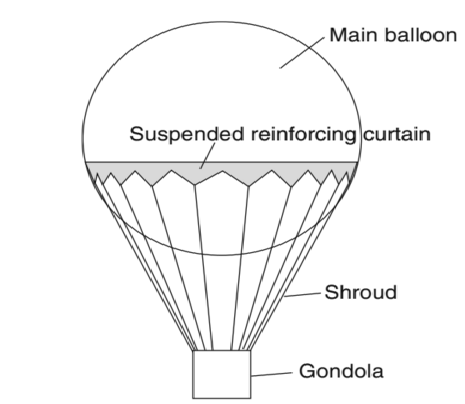
\includegraphics[width=0.5\textwidth]{figuras/balaoEsferico}
		\caption{Esquema de Balão Esférico com Fita de Carga.}
		\label{img:balaoEsferico}
	\end{figure}

	A fórmula para cálculo da tensão é a seguinte:

	$T = pr/2$ \\
	onde: \\
	\textbf{T} = tensão, \\ 
	\textbf{P} = pressão interna do balão, \\
	\textbf{R} = raio do balão. \\

\subsubsection{Sistema do Balão}

	Existem dois modelos de balões metereológicos empregados atualmente pela Agência Espacial Ameriacana (NASA) , o sistema Zero Pressão (ZP) e o Super-Pressão (SP). 
	
	O sistema ZP recebe esse nome porque a pressão interna do balão é a mesma  pressão do ambiente de atuação do sistema. Na parte de baixo do envelope do balão existe pelo menos um duto que permite a saída do gás dentro do balão para o alívio da pressão interna, como é exemplificado na Figura \ref{img:maiorBalaoZeroPressao}.

	maiorBalãoZeroPressao

	\begin{figure}[H]
		\centering
		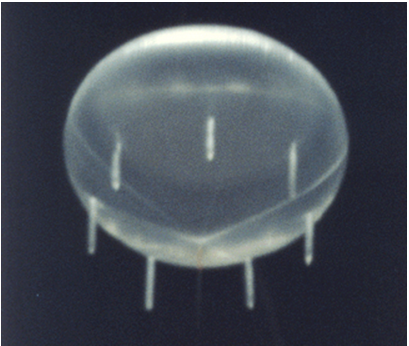
\includegraphics[width=0.5\textwidth]{figuras/maiorBalaoZeroPressao}
		\caption{Maior Balão Zero Pressão Usado pela NASA.}
		\label{img:maiorBalaoZeroPressao}
	\end{figure}

	Para esse sistema normalmente é utilizado um material com 20 micrometros de espessura para o envelope. O balão é inflado em terra e é solto na atmosfera até que a força de empuxo seja igual ao seu peso. O duto funciona de tal modo que quando a pressão interna na base do balão excede a pressão da atmosfera exterior, o duto é empurrado para fora e forma uma um cilindro que permite que parte do gás seja expelida. Quando a diferença de pressão é negativa, a pressão atmosférica empurra o duto para dentro, impedindo a entrada de ar. Com a queda de temperatura, o gás esfria e contrai-se, diminuindo o volume e consequentemente o empuxo. Em balões atmosféricos usado pela NASA, para manter a altitude constante durante a noite o balão solta pesos c, como por exemplo areia, durante esse período a quantidade de gás dentro do envelope é a mesma pois o duto se fecha quando o gás se contrai. Porém, no próximo dia, com o aumento da temperatura o gás irá se expandir, aumentando o volume e subindo mais, pois estará mais leve. Para manter uma altitude a mais constante possível, segundo a NASA, um balão desse tipo requer uma perda de 6 a 8\% de massa quando a temperatura diminui. O principal problema desse tipo de sistema é a perda de gás pelo duto aberto ao ambiente. 

	O sistema SP possui a vantagem de ser completamente vedado, ou seja, não perde gás durante seu período de atividade. Por esse fato o balão tem uma pressão interna maior que a pressão externa e isso implica no aumento da espessura do envelope, normalmente cerca de 10 vezes maior que a espessura de um balão ZP (Yajima, 2009). A Figura 3 mostra a distribuição de pressão de um balão atmosférico da NASA, percebe-se que o equador do envelope é a área de maior concentração de pressão e isso inviabilizaria o uso de uma fita de carga para fixar a payload, nesse tipo de balão a payload é fixada na parte de baixo do envelope, esse fato exige que a parte de fixação seja reforçada para que o envelope não seja danificado.

	distribuicaoPressao

	\begin{figure}[H]
		\centering
		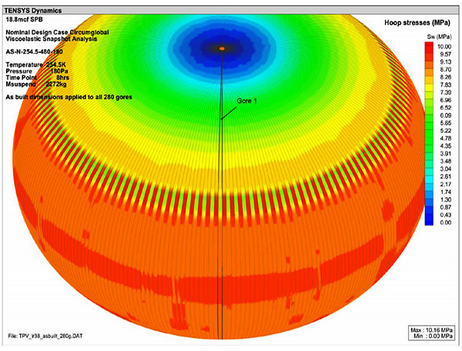
\includegraphics[width=0.5\textwidth]{figuras/distribuicaoPressao}
		\caption{Distribuição de Pressão de um Balão Super Pressão.}
		\label{img:distribuicaoPressao}
	\end{figure}

	Em linhas gerais o balão ZP é mais leve, porém possui o problema de perder gás durante sua operação. O balão SP tem a vantagem de não perder gás durante sua operação, porém é mais pesado pois precisa ter um envelope mais grosso, e não é possível o uso de uma fita de carga. Pelo fato de ser mais leve, o sistema empregado no projeto do Sistema Unificado de Monitoramento será o balão Zero Pressão. Deve-se calcular e analisar a perda diária de gás e como isso influenciará no empuxo do balão cativo.

	\subsubsection{Adaptação do Sistema de Balão para o SUM}

		Uma vez escolhido o sistema do balão deve-se adaptá-lo a um balão cativo. No caso de um balão preso ao chão o problema da perda de gás devido a variação da temperatura continua a mesma. Com o aumento da temperatura a pressão interna aumenta e pode fazer com que o gás vaze pelo duto, porém o balão não perde altitude desde que o Empuxo Líquido seja maior que zero ( o empuxo líquido é a força vertical resultante desconsiderando a tração nos cabos de sustentação). A pressão interna do balão é igual a pressão externa, com a variação da temperatura, a pressão do ar mantém-se aproximadamente constante.  Com a queda da temperatura, o gás contrai-se diminuindo o volume do balão e a pressão interna no instante de queda de temperatura é menor que a externa, desta forma o duto se fecha não permitindo a entrada de ar ou saída de gás, portanto a quantidade de matéria e a pressão dentro do envelope são aproximadamente constantes nessa fase. Usando a equação de \textit{Clapeyron}:

			$P1V1/T1 = P2V2/T2$

		com pressão constante, é possível descobrir a variação do volume do balão quando a temperatura diminui. Utilizando a base de dados do Instituto Nacional de Meteorologia (INMET) dos últimos 10 anos (entre 2005 e 2015) constata-se uma temperatura máxima média de 32ºC (305,15 K) e uma temperatura mínima média de 7.8ºC (281 K), temos o seguinte:

			 $V2/V1$ = 281/305,15  = $V2/V1$ = 0,92086

		Desta forma o volume final (V2) é cerca de 7,9% menor que o volume inicial (V1).
		
		Para o aumento da temperatura, ao expandir-se, o gás sai pelo duto mantendo o volume constante ( mesmo volume da queda de temperatura) , bem como a pressão aproximadamente constante, desta forma deve-se calcular a quantidade de gás perdida durante esse processo. Usando a Lei dos Gases ideais e adaptando-a para a situação temos:

			$PV = nRT$

		, como \textbf{P},\textbf{V} e \textbf{R} são constantes nesse processo temos a variação da quantidade de matéria em função da temperatura.

		$nT = cte  = n1T1 = n2T2  = n2/n1 = T1/T2$

		Sendo T1 a temperatura mais fria e T2 a temperatura mais quente, temos:

			$n2 = n1(T1/T2) = n2 = n1 (281/305,15) n2 = n1 (0,92086)$

		Logo, balão perde 7.9\% de gás por dia, podemos calcular a quantidade de matéria final após \textit{t} dias através da seguinte fórmula:

			$nf = ni (0,92086)^t$
			                                 
 		onde \textbf{nf} é a quantidade de matéria final, \textbf{ni} é a quantidade de matéria inicial e \textbf{t} é o número de dias.


% subsection modelo_do_bal_o (end)